% This file was created by matlab2tikz.
%
%The latest updates can be retrieved from
%  http://www.mathworks.com/matlabcentral/fileexchange/22022-matlab2tikz-matlab2tikz
%where you can also make suggestions and rate matlab2tikz.
%

\documentclass[]{standalone}
\usepackage{amsmath}
\usepackage{graphicx}
\usepackage[pdf]{pstricks}
\usepackage{pgfplots}
\pgfplotsset{compat=newest}
\usepgfplotslibrary{fillbetween}
%% the following commands are needed for some matlab2tikz features
\usetikzlibrary{plotmarks}
\usetikzlibrary{arrows.meta}
\usepgfplotslibrary{patchplots}
\usetikzlibrary{decorations.text}
\usetikzlibrary{shapes.multipart}
%\usetikzlibrary{external}
%\tikzexternalize % activate!

\begin{document}
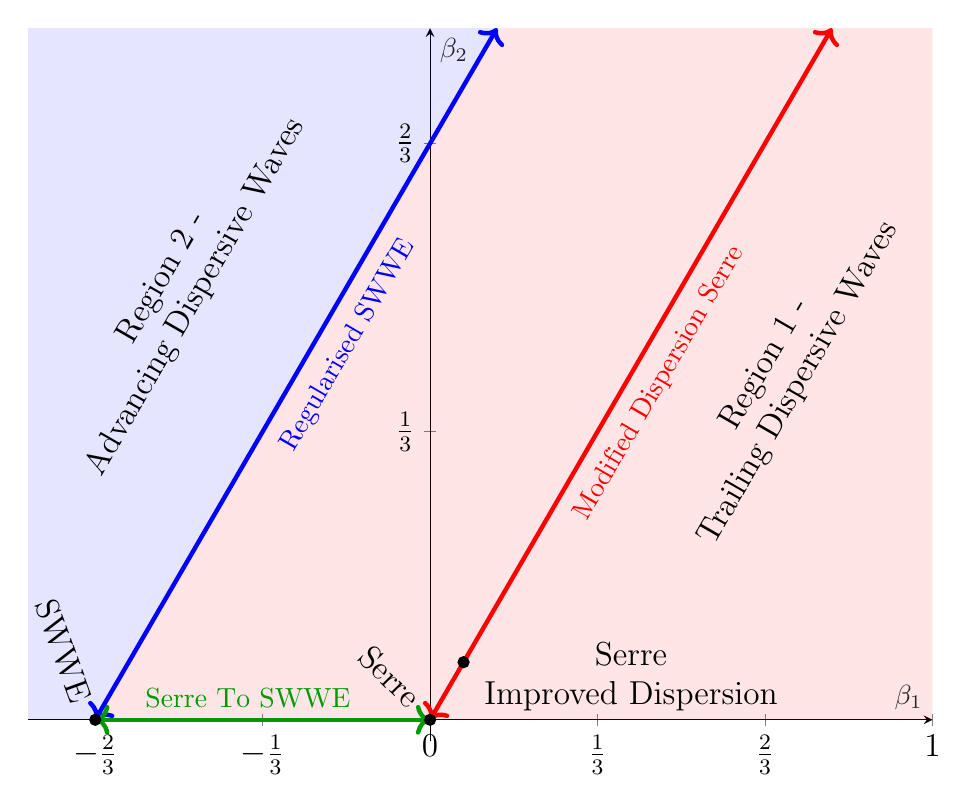
\begin{tikzpicture}[every text node part/.style={align=center}]
\tikzstyle{every node}=[font=\large]
\begin{axis}[%
width=4.521in,
height=3.566in,
at={(0.758in,0.481in)},
scale only axis,
axis x line = middle,
axis y line = middle,
xmin=-0.8,
xmax=1,
xtick={-1,-0.66666,-0.33333,0.33333,0.66666,1},
xticklabels = {$-1$,$-\frac23$,$-\frac13$,$\frac13$,$\frac23$,$1$},
extra x ticks={0},
xlabel style={font=\color{white!15!black}},
xlabel={$\beta_1$},
ymin=-0.025,
ymax=0.8,
ytick={0.33333,0.66666,1,1.33333},
yticklabels = {$\frac13$,$\frac23$,$1$,$\frac43$},
ylabel style={font=\color{white!15!black}},
ylabel={$\beta_2$},
axis background/.style={fill=white},
];
\addplot+[name path=Above,mark=none, draw=none] coordinates {(-3,0) (-10,0)};

\draw[<->,blue,ultra thick] (0.13333,0.8) --   (-0.66666,0) ;
\addplot[draw=none,blue,decoration={text along path,
	text={Regularised SWWE},
	raise=-3ex,
	text color={blue},
	text align={left indent={0.5\dimexpr\pgfdecoratedpathlength\relax}}},
postaction={decorate}]
coordinates {(-1.66666,-1) (1,1.66)};

\path[name path=Critical ] (-0.66666,0) -- (1,1.66) ;


\addplot+[name path=Below,mark=none, draw=none] coordinates {(-2,0) (2,0)};
\addplot[blue,opacity=0.1] fill between[of=Above and Critical];
\addplot[red,opacity=0.1] fill between[of=Critical and Below];

\node[rotate = 60] at (axis cs: 0.7,.4) {Region 1 - \\ Trailing Dispersive Waves };
\node[rotate = 60] at (axis cs: -0.5,0.5) {Region 2 - \\ Advancing Dispersive Waves};

\draw[<->,red,ultra thick] (0,0) --   (0.8,0.8) ;

\addplot[draw=none,blue,decoration={text along path,
	text={Modified Dispersion Serre},
	raise=-3ex,
	text color={red},
	text align={left indent={0.25\dimexpr\pgfdecoratedpathlength\relax}}},
postaction={decorate}]
coordinates {(0,0) (1,1)};

\draw[<->,green!60!black,ultra thick] (-0.6666,0) --   (0,0) ;

\addplot[draw=none,decoration={text along path,
	text={Serre To SWWE},
	raise=1ex,
	text color={green!60!black},
	text align={left indent={0.15\dimexpr\pgfdecoratedpathlength\relax}}},
postaction={decorate}]
coordinates {(-0.6666,0) (0,0)};

\node[rotate = -45] at (axis cs: -0.08,0.05) {Serre};
\node[] at (axis cs: 0.4,0.05) {Serre \\Improved Dispersion};

\addplot[only marks] coordinates {(0,0) (-0.6666,0) (0.06666,0.06666)};
\node[rotate=-70] at (axis cs: -0.73,0.08) {SWWE};


\end{axis}

\end{tikzpicture}%

\end{document}